\chapter{Wstęp}
\section{Wstęp}
\paragraph{}
Celem projektu było stworzenie aplikacji webowej umożliwiającej tworzenie ankiet i nagradzanie użytkowników kuponami na produkty i usługi w zamian za ich wypełnienie.
\paragraph{}
Aplikacja pozwala firmom na tworzenie ankiet i zbieranie statystyk na temat udzielonych odpowiedzi, natomiast niezarejestrowani jako firma użytkownicy mają możliwość wypełnienia ankiety przy użyciu aplikacji webowej, bądź aplikacji mobilnej, w zamian za co otrzymają interesujący ich kupon. Każdy użytkownik ma gwarancję otrzymania nagrody w zamian za wypełnienie ankiety dzięki zastosowaniu rezerwacji kuponów. Statystyki pozwalają firmie określić najpopularniejsze odpowiedzi i wyznaczyć trendy wśród badanych grup wiekowych i narodowości.

\paragraph{}
Dokumentacja składa sie z czterech rozdziałów. W dalszej części rozdziału pierwszego scharakteryzowano założenia funkcjonalne i niefunkcjonalne systemu. W rozdziale drugim przedstawiono analizę problemu. Omówiono w nim problemy związane z tworzeniem systemu zapewniającego dane funkcjonalności, a także przedstawiono rozwiązania użyte w innych systemach o podobnych założeniach funkcjonalnych i niefunkcjonalnych. W rozdziale trzecim przedstawiono szczegółowy projekt systemu wraz z diagramami w notacji UML, pomagającymi zrozumienie zależności między komponentami systemu i wspomagającymi opis procesu działania aplikacji. W tym rozdziale przedstawiono również technologie zastosowane do stworzenia systemu, dzięki którym mógł on być napisany w sposób bardziej nowoczesny i efektywny. Opisane zostały również możliwości rozwoju i modyfikacji systemu. W rozdziale czwartym omówiono implementację systemu wraz z opisem kodu. Został tam szczegółowo opisany proces działania systemu z naciskiem na spójność między poszczególnymi komponentami.


\section{Specyfikacja wymagań}
\subsection{Założenia funkcjonalne}
\paragraph{}
System pozwala firmie na założenie konta, którym będzie reprezentowana w serwisie. Możliwe jest również odzyskiwanie hasła przy użyciu adresu e-mail podanego w czasie rejestracji. Firma może utworzyć w systemie ankietę oraz powiązać ją z kuponem na wybraną przez siebie usługę lub produkt. Po powiązaniu kuponu z ankietą firma może dodać do kuponu dowolną ilość kodów promocyjnych, które będą dystrybuowane w zamian za wypełnienie ankiety. Firma może również przeglądać statystyki dotyczące wypełnionych ankiet, które zapewniają informacje o procentowym rozkładzie odpowiedzi na dane pytanie oraz o wieku oraz narodowości wypełniającego. Ponadto firma ma możliwość przeglądania poszczególnych wypełnionych ankiet. Firma ma także możliwość przeglądania wszystkich swoich ankiet w systemie oraz usuwania poszczególnych ankiet oraz edycji, dodawania oraz usuwania kuponów. Firma może również trwale usunąć konto z systemu. Wypełniający ankiety może wypełnić ankietę za pomocą aplikacji webowej, bądź aplikacji mobilnej i w prosty sposób otrzymać kupon drogą mailową lub bezpośrednio na ekranie urządzenia po przesłaniu odpowiedzi.

\subsection{Założenia niefunkcjonalne}
\paragraph{}
Proces logowania, rejestracji i odzyskiwania hasła jest bezpieczny dla firmy i nie grozi utratą jakichkolwiek wrażliwych danych. Ankiety mogą zawierać różne rodzaje pytań i w trakcie ich tworzenia firma powinna mieć łatwość ich bieżącej edycji. Interfejs graficzny aplikacji webowej i mobilnej powinien być lekki i nowoczesny, o spójnej szacie kolorystycznej. Firma powinna mieć łatwość przeglądania swoich ankiet w systemie i pozwiązanych z nimi ankiet. Użytkownicy powinni być anonimowi w systemie, a dane przekazywane firmie powinny uniemożliwiać identyfikację poszczególnych osób, udzielających odpowiedzi na ankiety. Użytkownik powinien mieć możliwość łatwego wyboru ankiety z jasno określoną nagrodą w zamian za jej wypełnienie. Użytkownik powinien mieć również gwarancję otrzymania nagrody nawet w przypadku ograniczonej ilości kodów promocyjnych związanych z danym kuponem.

\paragraph{}
Funkcjonalności ze względu na użytkowników można również przedstawić w formie diagramu UML przypadków użycia.
\begin{figure}[h]
\centering
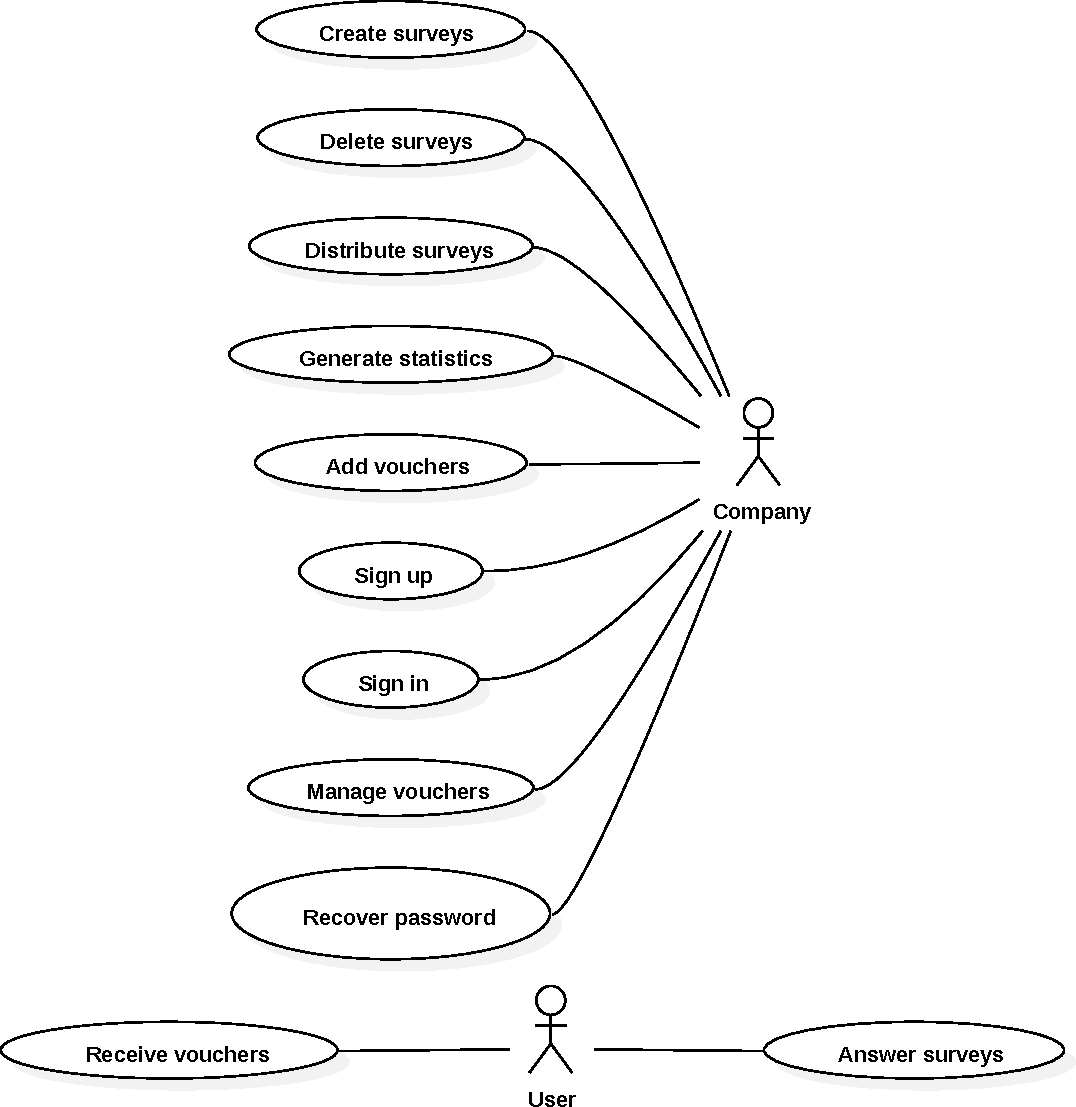
\includegraphics[width=10cm,height=10cm,keepaspectratio]{useCasePdf}
\caption{Diagram przypadków użycia dla systemu.}
\end{figure}

\paragraph{}
W dalszej części dokumentacji będą używane terminy, których znaczenie znajduje swój odpowiednik w modelu systemu. Terminy te zostaną teraz opisane dla zwiększenia czytelności i jasności dokumentacji:
\begin{itemize}
\item \textbf{Ankieta} - zbiór pytań otwartych, ze skalą lub jednokrotnego/wielokrotnego wyboru.
\item \textbf{Kupon} - zniżka na konkretny produkt lub usługę.
\item \textbf{Kod promocyjny} - kod powiązany z kuponem, uprawniający do zniżki na konkretny produkt lub usługę.
\end{itemize}
\clearpage